\documentclass[handout, aspectratio=169]{beamer}

\usepackage[frenchb]{babel}
\usepackage[T1]{fontenc}
\usepackage[utf8x]{inputenc}
 
\usetheme{Berkeley}
\usecolortheme{dove}
\usecolortheme{seahorse}
\useinnertheme{rounded}

\def\restriction#1#2{\mathchoice
              {\setbox1\hbox{${\displaystyle #1}_{\scriptstyle #2}$}
              \restrictionaux{#1}{#2}}
              {\setbox1\hbox{${\textstyle #1}_{\scriptstyle #2}$}
              \restrictionaux{#1}{#2}}
              {\setbox1\hbox{${\scriptstyle #1}_{\scriptscriptstyle #2}$}
              \restrictionaux{#1}{#2}}
              {\setbox1\hbox{${\scriptscriptstyle #1}_{\scriptscriptstyle #2}$}
              \restrictionaux{#1}{#2}}}
\def\restrictionaux#1#2{{#1\,\smash{\vrule height .8\ht1 depth .85\dp1}}_{\,#2}}

\def\derPar#1#2{\frac{\partial #1}{\partial #2}}

\title[Shape Opti. Waveguides]{Présentation d’un article :\\ On shape optimization of optical waveguides using inverse problem techniques \\\small{Thomas Felici \& Heinz W Engl}}
\author{Alexandre \bsc{Vieira}}
\institute{INSA de Rouen}
\date{\today}


\AtBeginSection[]
{
	\begin{frame}
		\frametitle{Sommaire}
		\tableofcontents[currentsection, hideothersubsections]
	\end{frame}
}

\begin{document}

\begin{frame}
\titlepage
\end{frame}

\begin{frame}
	\frametitle{Sommaire}
	\tableofcontents
\end{frame}

\section{Formulation du problème}
\begin{frame}
	\frametitle{Équation étudiée}
	\[\Delta U+n^2U=0\]
	\begin{figure}[!h]
	\centering
	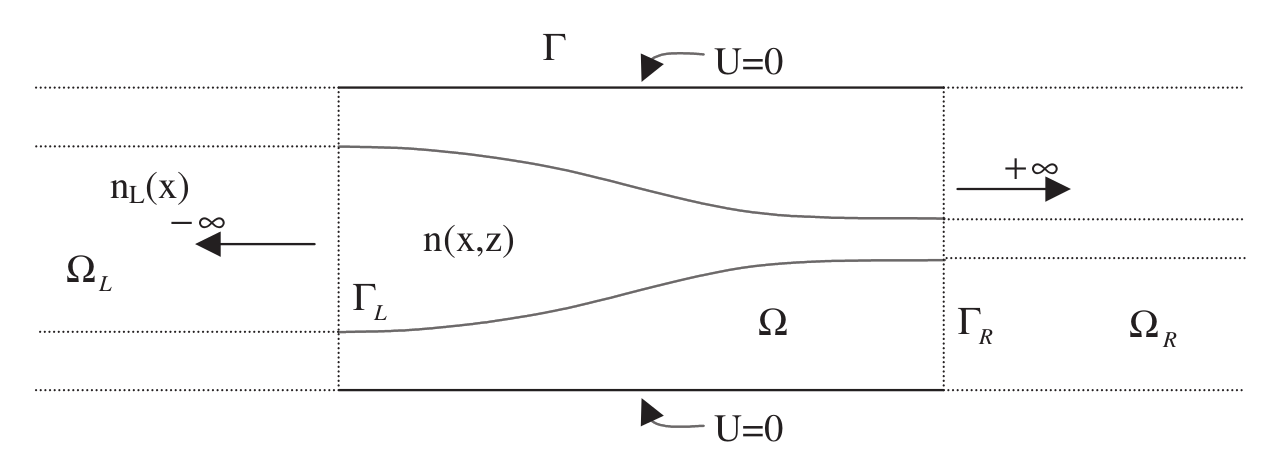
\includegraphics[scale=0.22]{images/waveguide-Taper.png}
	\caption{Profil du taper}
	\label{fig:Profil}
\end{figure}
\end{frame}

\begin{frame}
	\frametitle{Recherche de conditions au bord}
	\begin{center} 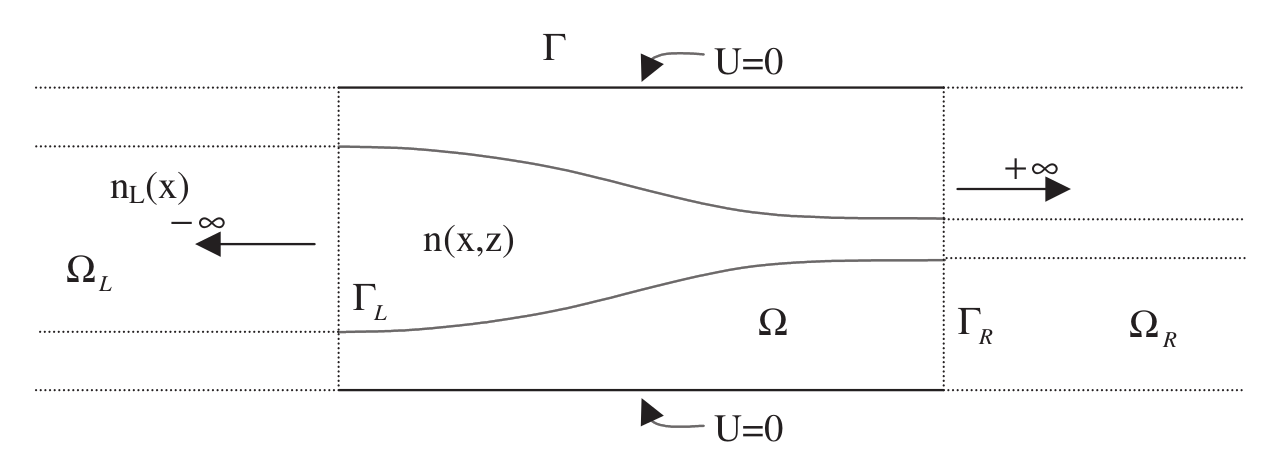
\includegraphics[scale=0.10]{images/waveguide-Taper.png} \end{center}
\begin{equation} \label{eq10} \scalebox{0.65}{$
\left\{\begin{array}{r c l r}
	\Delta U + n^2U&=&0 &\text{pour } (x,z)\in\Omega\\
	\restriction{U}{\Gamma}&=&0 &\text{(murs réfléchissants)}\\
	\frac{\partial U}{\partial z}+i\sum_{k=1}^\infty {\beta_k^{(L)}}^2\left\langle U,\tilde{U}^{(L)}_k\right\rangle \tilde{U}^{(L)}_k &=& 2i\sum_{k=1}^\infty {\beta_k^{(L)}}^2 \left\langle U_I,\tilde{U}_k^{(L)}\right\rangle\tilde{U}^{(L)}_k &\text{sur }\Gamma_L\\
	\frac{\partial U}{\partial z}-i\sum_{k=1}^\infty {\beta_k^{(R)}}^2 \left\langle U,\tilde{U}_k^{(R)} \right\rangle \tilde{U}_k^{(R)}&=&0 &\text{sur } \Gamma_R
\end{array}\right.$}
\end{equation}
\end{frame}

\begin{frame}
	\frametitle{Problème d'optimisation}
\begin{equation} \label{eq7} \langle \tilde{U}_k,\tilde{U}_k\rangle = \frac{1}{\beta_k} \end{equation}
On cherche à maximiser :
\begin{equation}\label{eq11} P(n^2)=\beta_1^2|\langle U,\tilde{U}_1^{(R)}\rangle|^2=\beta_1^2\left|\int_{x\in\Gamma_R} U(x,z_R)\tilde{U}_1^{(R)}(x)dx\right|^2\end{equation}
$\Rightarrow$Formulation difficile à exploiter.
\end{frame}

\section{Solution du problème direct}
\begin{frame}
	\frametitle{Représentation locale}
\[L_t(U)=\frac{\partial^2U}{\partial x^2}+n^2(x,z)U\]
\begin{equation} \label{eq13}
	\begin{array}{c c c c}
		L_t(U_k)&=&\beta_k^2U_k &\text{dans } \Omega_z\\
		\restriction{U_k}{\partial\Omega_z}&=&0
	\end{array}
\end{equation}
\begin{equation}\label{eq14}
\begin{array}{c c l}
U&=&\sum_{k=1}^\infty (a_k+a_{-k})U_k\\
\frac{\partial U}{\partial z}&=&\sum_{k=1}^\infty (a_k-a_{-k})i\beta_kU_k
\end{array}
\end{equation}
\end{frame}

\begin{frame}
	\frametitle{Représentation locale}
Puissance dans le $k$ème mode : $|a_k|^2$ et $|a_{-k}|^2$. Ainsi :
\[P(n)=|a_1|^2\]
Longue démonstration pour avoir :
\begin{equation} \label{eq17}
\dot{a}_k(z)-i\beta_ka_k(z)=\sum_{j\neq k,0} r_{kj}(z)a_j(z),\ k\neq 0
\end{equation}
avec $\beta_{-k}=-\beta_k$ et \[r_{kj}(z)=\frac{\int_{\Omega_z} \frac{\partial n^2}{\partial z} U_kU_j ds}{2(\beta_k-\beta_j)}\]
pour tout $j\neq k$, $j,k\neq 0$\\
\end{frame}

\section{Résultats numériques et interprétation}
\begin{frame}
	\frametitle{Discrétisation}
\begin{figure}[!h]
	\centering
	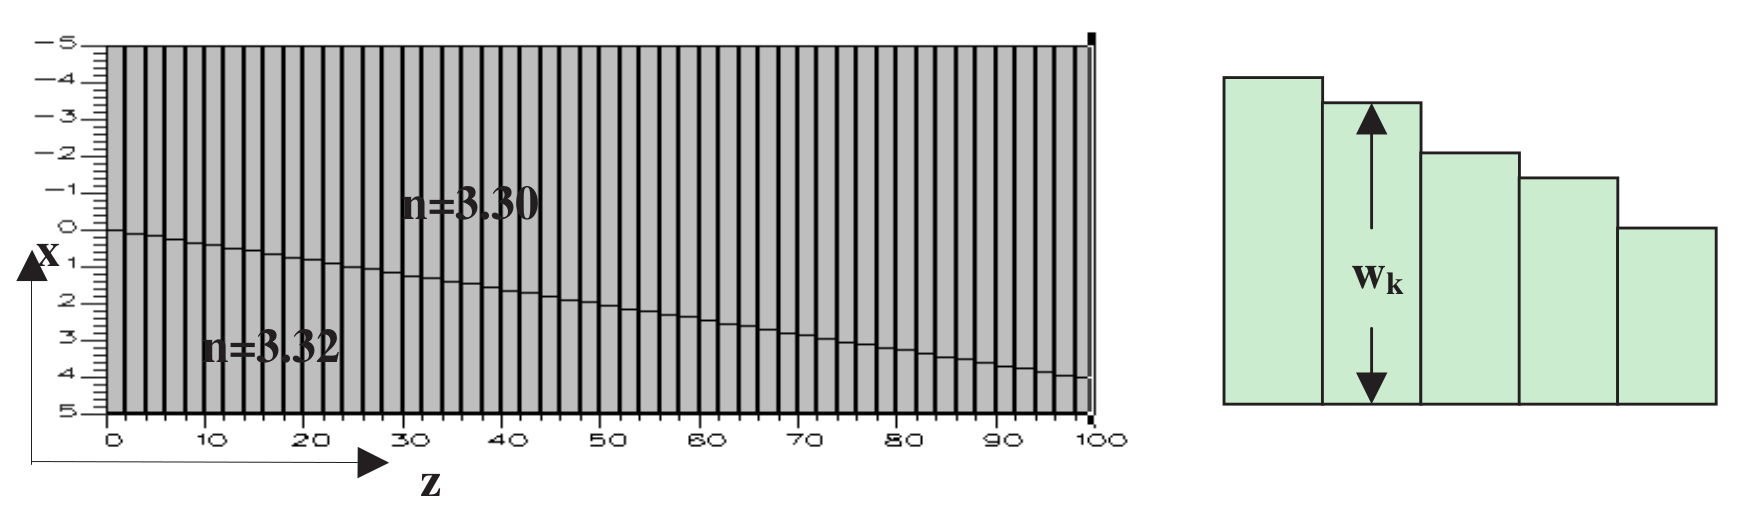
\includegraphics[scale=0.15]{images/numOpti.png}
	\caption{Profil du taper : discrétisation pour le problème d'optimisation}
	\label{fig:numOpti}
\end{figure}
\end{frame}

\begin{frame}
	\frametitle{Résultats numériques}
\begin{figure}[!h]
	\centering
	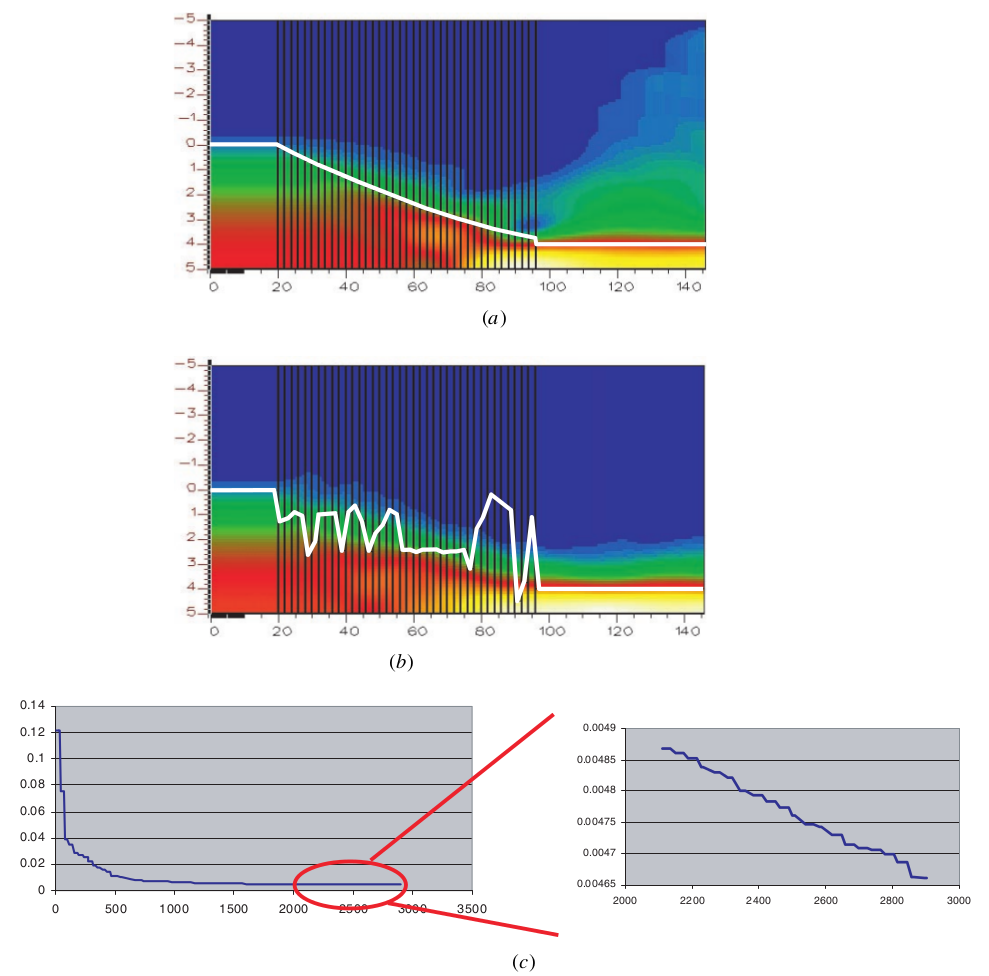
\includegraphics[scale=0.175]{images/result48.png}
	\caption{Profil du taper : résultat avec $N=48$. (a) Forme initial du taper (b) Forme optimale (c) Perte d'énergie en fonction du nombre d'itérations.}
	\label{fig:result48}
\end{figure}
\end{frame}

\begin{frame}
	\frametitle{Résultats numériques}
\begin{figure}[!h]
	\centering
	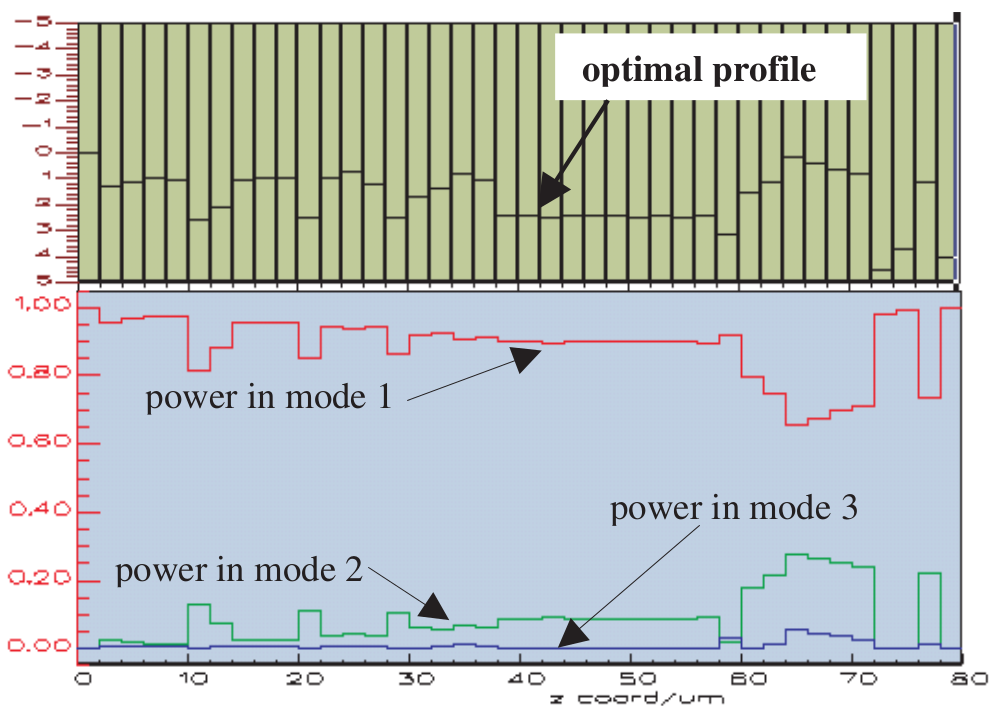
\includegraphics[scale=0.22]{images/powMode.png}
	\caption{L'énergie est préservée grâce à la resonnance avec les autres modes}
	\label{fig:powMode}
\end{figure}
\end{frame}

\begin{frame}
	\frametitle{Un problème mal posé}
\begin{itemize}
	\item Variations arbitrairement grandes sur l'indice de refraction $n$ $\Rightarrow$ Une solution $U$ toujours aussi proche qu'on veut.
	\item Or, dans l'algorithme d'optimisation, la fonction objectif et les contraintes ne dépendent que de $U$, et non de $n$ !
	\item Point de vue physique : l'onde ne voit pas les pics plus petites que sa longueur d'onde
	\item Pour gagner en stabilité : réduire l'espace de recherche (ajouter de la continuité par exemple)
	\item À contrario, on pourrait plutôt essayer de chercher la distribution des indices provenant d'une certaine mesure.
\end{itemize}
\[\Rightarrow \text{ approche problème inverse}\]
\end{frame}

\section{Approche par problèmes inverses}
\begin{frame}
	\frametitle{Formulation du problème}
\[1=\sum_{k\in RB} |a_{-k}(0)|^2 + \sum_{k\in RB} |a_k(z_R)|^2 \]
\[\text{avec } RB=\{k\in \mathbb{Z}^* | \beta_k^2>0\}\]
Pour rappel :
	\[U(x,z_R)=\sum_{k=1}^\infty a_k(z_R)U_k^{(R)}(x)\]
Égalité seulement si :
\begin{equation}\label{eq23}
	\begin{bmatrix} |a_1(z_R)| \\ |a_2(z_R)| \\ |a_3(z_R)| \\ \vdots \end{bmatrix} = \begin{bmatrix} 1 \\ 0 \\ 0 \\ \vdots \end{bmatrix}
\end{equation}
\end{frame}

\begin{frame}
	\frametitle{Formulation du problème}
Avantage numérique : on prend en compte tous les $a_k$ !\\
Dépendance non linéaire de $n$, et pas forcément de solution. D'où : approche par moindre carrés, et utilisation de la méthode de Newton.
\begin{equation}\label{eq24}
	\restriction{\frac{\partial\mathbf{a}}{\partial n}}{n}\delta n=\mathbf{a}_1-\mathbf{a}(n)
\end{equation}
\end{frame}

\begin{frame}
	\frametitle{Formulation du problème}
	\[\restriction{\frac{\partial\mathbf{a}}{\partial n}}{n}=UDV^T\]
Instabilité numérique reglé par troncature des valeurs singulières du jacobien : choix de $0<\alpha<1$ et :
	\[r:=\max\{i | d_i\geq \alpha d_1\}\]
Et :
	\[D_{red}=diag(d_1,...,d_r,0,...,0)\]
\begin{equation}\label{eq26}
	\delta n=VD_{red}^\dagger U^\dagger [\mathbf{a}_1-\mathbf{a}(n)]
\end{equation}
\end{frame}

\begin{frame}
	\frametitle{Formulation du problème}
	\[\min F(\lambda)=\|\mathbf{a}_1-\mathbf{a}(n_k+\lambda\delta n)\|_2^2\]
	\[n_{k+1}=n_k+\lambda_{min}\delta n\]
\begin{figure}[!h]
	\centering
	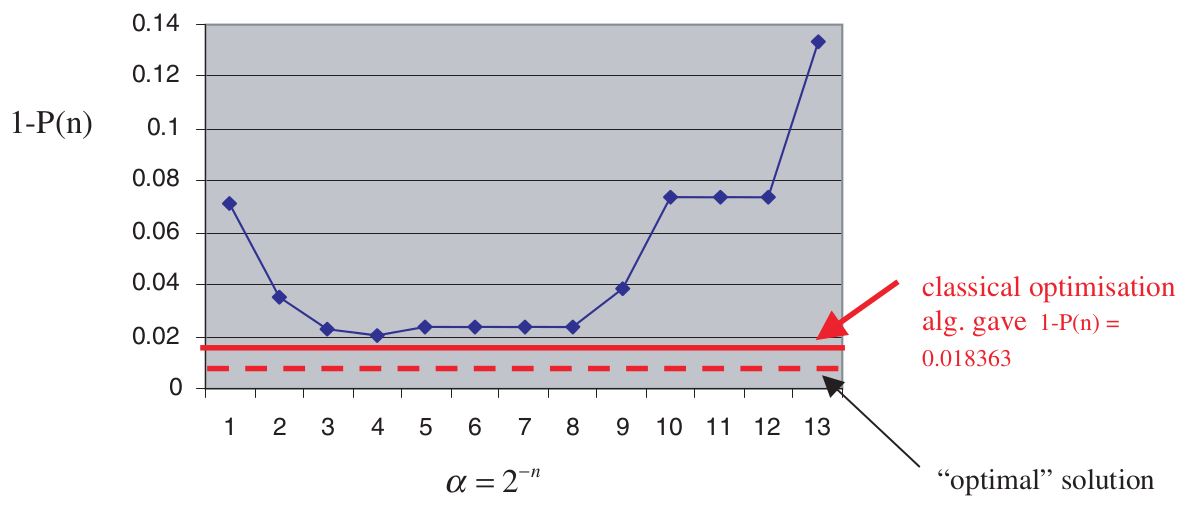
\includegraphics[scale=0.14]{images/convAlgo13.png}\\
	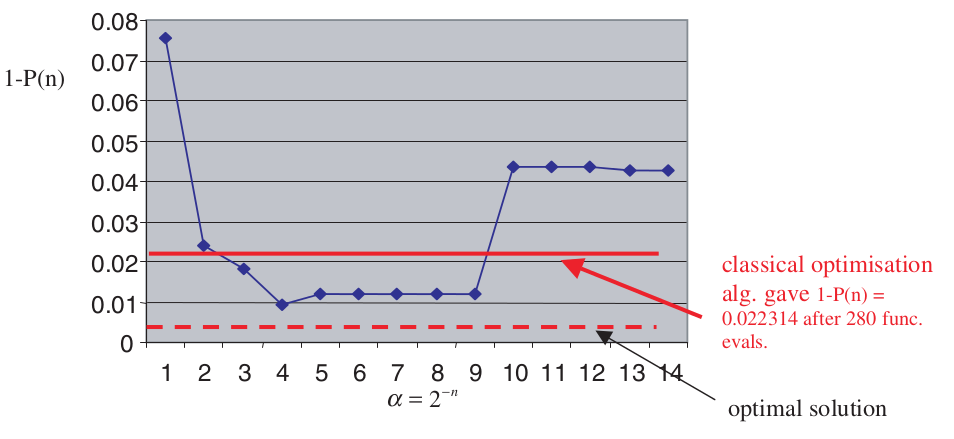
\includegraphics[scale=0.16]{images/convAlgo48.png}
	\caption{(1) N=13, M=10 modes (2) N=48, M=15}
	\label{fig:accConv}
\end{figure}
\end{frame}

\section*{Conclusion}
\begin{frame}
	\frametitle{Conclusion}
\begin{itemize}
	\item Une approche par problème inverse efficace, mais sous certaines contraintes
	\item Moyen d'améliorer : algorithme en cascade
	\item Calculs très formels : il manque parfois quelques considérations mathématiques (notamment sur les séries)
\end{itemize}
\end{frame}

\end{document}
